\labday{30 March 2023}

\experiment{PPDr}

The PPD was re-assembled for testing, the trigger PMT was re-connected. A new pump was fitted since the old one was broken by (suspected) water ingress. The flow of the pump was adjusted until \SI{6}{\litre\per\minute} was shown on the gilibrator flow-meter. Droplets were observed on the detector nicely :)

\begin{figure}[H]
\begin{center}
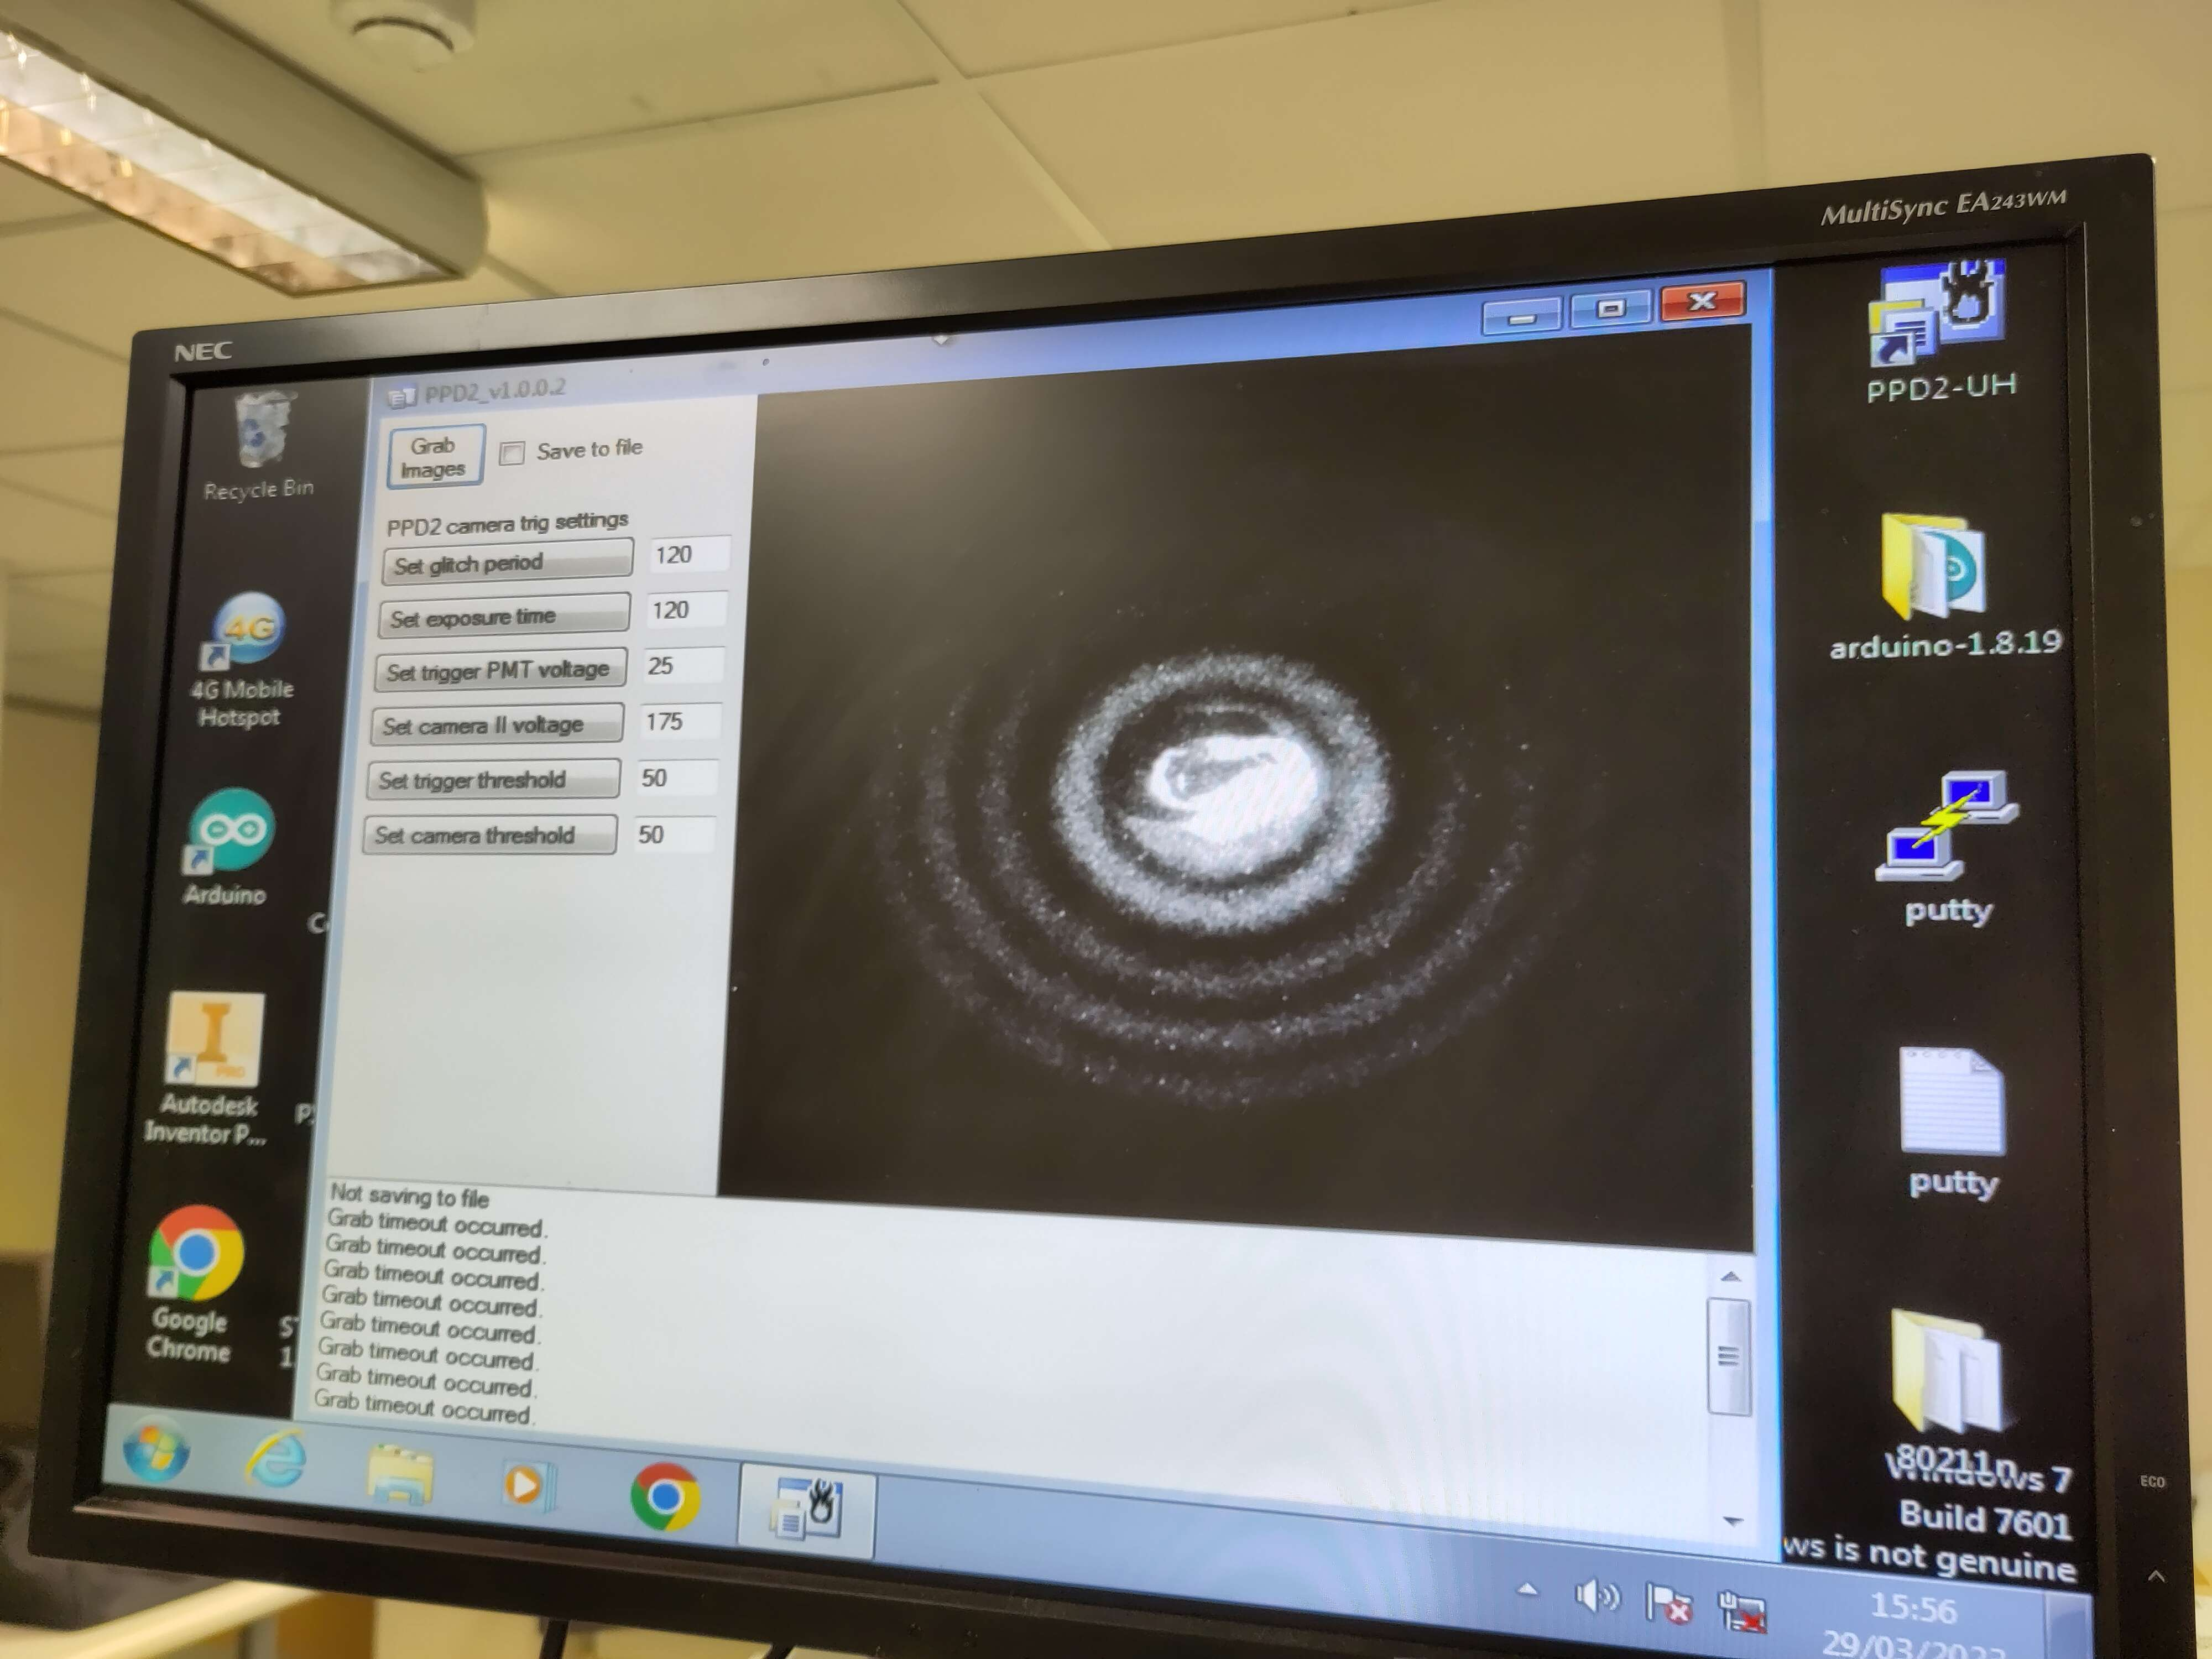
\includegraphics[width=0.5\linewidth]{Figures/PPDDropletImage}
\end{center}
\caption{Image of droplet scattering.}
\label{fig:PPDDropletImage}
\end{figure}

Ther eis still a huge problem with the computer images. There is a grab timeout which seems to randomly occur. Using a new computer with a firewire port which does not go through a PCI slot fixed the issue. It was determined that waiting for the latte-panda computer to arrive would be the preferable option for the new system. In addition, it was determined that transfering the PPD to a new case was the preferable option.
